%══════════════════════════════════════════════════════════════════════
\chapter{Thermo-fluid Systems}
\label{ch:thermofluid}
%══════════════════════════════════════════════════════════════════════

Thermodynamics is the \textbf{universal science of physical processes}: every
model constructed so far --- mechanical, electrical, hydraulic, thermal ---
can be studied through its lens.  When C- and I-fields are constrained to
conserve energy, or R-fields are arranged to dissipate power, thermodynamic
arguments are implicitly at work.  Most dynamic models can be characterised
as \textbf{isothermal models}, and much of engineering thermodynamics is
concerned with changes between equilibrium states rather than with the
transient path of change.  When the path itself is relevant --- when we care
about irreversibility and entropy production --- we enter the domain of
\textbf{irreversible thermodynamics}, which involves genuinely non-equilibrium
systems.

The modelling strategy adopted here rests on the assumption that physical
extents and time scales are such that \textbf{local pseudo-equilibrium
conditions} exist: at each instant every identifiable lump of substance can
be treated as if it were in thermodynamic equilibrium, even if the overall
system is not.  Under this assumption it becomes possible to define
meaningful state variables at every instant and to write first-order ODEs for
their evolution.

This chapter develops two complementary threads: the \emph{true bond-graph
representation} of thermodynamic systems (which identifies temperature $T$ as
an effort and entropy rate $\dot{S}$ as a flow, so that $T\dot{S}$ is genuine
power), and a critical re-examination of \emph{fluid-dynamic systems},
including the lumped modelling of fluid inertia and compliance, Bernoulli's
equation, and the challenges introduced by compressibility and mass exchange
through a control volume.

%──────────────────────────────────────────────────────────────────────
\section{Basic thermodynamics in true bond-graph form}
\label{sec:true_bg_thermo}
%──────────────────────────────────────────────────────────────────────

\subsection{Assumptions and notation}
\label{ssec:thermo_assumptions}

We begin with a set of simplifying assumptions that frame the entire
discussion:
\begin{itemize}[leftmargin=2em,itemsep=4pt]
  \item \textbf{Closed system (Lagrangian viewpoint).}  No mass passes
    through the boundary.  The total mass $m$ of the substance is fixed.
  \item \textbf{Pseudo-equilibrium.}  All parts of the substance are at
    essentially identical conditions of pressure, temperature, and density,
    so that a single set of state variables describes the whole lump.
  \item \textbf{No motion, no electromagnetic or surface-tension forces.}
    Under these conditions a \emph{pure substance} has only
    \textbf{two independent properties}; all others are given by the
    \emph{equations of state}.
\end{itemize}

Extensive quantities (volume, internal energy, entropy) for a \emph{unit
mass} are written in lowercase: $v$ (specific volume), $u$ (specific
internal energy), $s$ (specific entropy).  When a mass $m$ of the substance
is involved the corresponding total quantities are:
\begin{equation}
  V = mv, \qquad U = mu, \qquad S = ms.
  \label{eq:extensive}
\end{equation}


\subsection{The Gibbs equation and the internal energy function}
\label{ssec:gibbs}

It is assumed that the \textbf{internal energy per unit mass} $u$ is a
function of the \emph{specific volume} $v$ and the \emph{specific entropy}
$s$:
\begin{equation}
  u = u(v, s).
  \label{eq:int_energy}
\end{equation}
The \textbf{Gibbs equation} relates infinitesimal changes in $u$ to
changes in $v$ and $s$:
\begin{equation}
  \mathrm{d}u = T\,\mathrm{d}s - p\,\mathrm{d}v,
  \label{eq:gibbs}
\end{equation}
where $T$ is the \emph{thermodynamic temperature} (conjugate to entropy)
and $p$ is the \emph{pressure} (conjugate to volume, with a sign because
expansion does work on the surroundings).  In rate form:
\begin{equation}
  \frac{\mathrm{d}u}{\mathrm{d}t}
  = T\,\frac{\mathrm{d}s}{\mathrm{d}t} - p\,\frac{\mathrm{d}v}{\mathrm{d}t}.
  \label{eq:gibbs_rate}
\end{equation}
The first term ($T\dot{s}$) is associated with a flow of heat or,
sometimes, with dissipative work; the second term ($p\dot{v}$) is
associated with \emph{reversible} mechanical power.

Comparing \eqref{eq:gibbs} with the total differential
$\mathrm{d}u = (\partial u/\partial s)\,\mathrm{d}s
+ (\partial u/\partial v)\,\mathrm{d}v$
immediately identifies:
\begin{equation}
  T = \frac{\partial u}{\partial s}, \qquad
  -p = \frac{\partial u}{\partial v}.
  \label{eq:gibbs_partials}
\end{equation}
A useful consistency check is the \textbf{Maxwell reciprocal relation},
which follows from the symmetry of mixed second partial derivatives:
\begin{equation}
  \left.\frac{\partial T}{\partial v}\right|_{s}
  = \frac{\partial^{2}u}{\partial v\,\partial s}
  = \left.\frac{\partial(-p)}{\partial s}\right|_{v}.
  \label{eq:maxwell}
\end{equation}


\subsection{The pure substance as a true bond-graph C-field}
\label{ssec:cfield}

The constitutive laws of the pure substance may be represented by a
\textbf{true bond-graph C-field}, where $T$ and $p$ are the \emph{efforts}
and $s$ and $v$ are the \emph{displacements}:


\begin{figure}
  \centering
  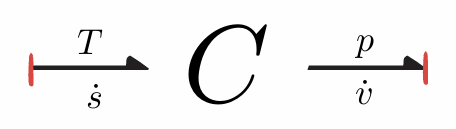
\includegraphics[width=0.6\textwidth]{figs/chapter8/8_1.png}
  \caption{True bond-graph C-field for the pure substance}
\end{figure}



The identification of $T$ as an effort and $s$ as a displacement is the
crucial distinction between a \textbf{true bond graph} and the
\textbf{pseudo-bond graph}: in the true formulation $T\dot{s}$ is genuine
thermodynamic power, whereas in the pseudo-bond graph the product of
conjugate variables is merely a useful analogy (heat flow $\dot{Q}$) and
not a true power.

Under \textbf{integral causality} the C-field is expressed as:
\begin{equation}
  T = T(s, v), \qquad p = p(s, v),
  \label{eq:cfield_integral}
\end{equation}
i.e.\ the efforts are computed from the stored displacements.  For
\emph{mixed-} or \emph{all-derivative causality} the constitutive laws
must be switched around, expressing the displacements as functions of the
efforts.  This inversion is accomplished systematically through the
\textbf{Legendre transformations} of the internal energy $u$.


\subsection{Legendre transformations and causal patterns}
\label{ssec:legendre}

Different causal patterns at the two ports of the C-field correspond to
different Legendre transforms of $u$:

\paragraph{Enthalpy.}  Replace $s$ (displacement) by $p$ (effort) as
independent variable:
\begin{equation}
  h(s, p) = u + pv,
  \qquad
  \frac{\partial h}{\partial s} = T(s,p),
  \qquad
  \frac{\partial h}{\partial p} = v(s,p).
  \label{eq:enthalpy}
\end{equation}
Here the $T$-port retains integral causality ($T$ computed from $s$) while
the $p$-port has derivative causality ($p$ is now an input, $v$ an output).

\paragraph{Helmholtz free energy.}  Replace $s$ by $T$:
\begin{equation}
  f(T,v) = u - Ts,
  \qquad
  \frac{\partial f}{\partial T} = -s(T,v),
  \qquad
  \frac{\partial f}{\partial v} = -p(T,v).
  \label{eq:helmholtz}
\end{equation}

\paragraph{Gibbs free energy.}  Replace both $s$ by $T$ and $v$ by $p$:
\begin{equation}
  \phi(T,p) = u + pv - Ts,
  \qquad
  \frac{\partial \phi}{\partial T} = -s(T,p),
  \qquad
  \frac{\partial \phi}{\partial p} = v(T,p).
  \label{eq:gibbs_free}
\end{equation}

\begin{insightbox}[Why use state functions?]
  Constitutive laws can in principle be written without reference to any
  state function.  The danger is that \emph{arbitrary} constitutive laws
  would not, in general, allow the existence of an internal energy function:
  a substance with such laws could, in a cycle, produce net energy and thus
  act as a \emph{perpetual motion machine of the first kind}.  Deriving
  constitutive laws by differentiating $u$, $h$, $f$, or $\phi$ is therefore
  always safer, since conservation of energy is \emph{automatically} built
  into the relations.  The C-field derived from a Legendre transform is
  guaranteed to be conservative.
\end{insightbox}


\subsection{The perfect gas: Helmholtz free energy route}
\label{ssec:perfect_gas}

A classical example of a constitutive law \emph{not} stated in terms of
state-function derivatives is the \textbf{perfect gas law} (per unit mass):
\begin{equation}
  pv = RT,
  \label{eq:perfect_gas}
\end{equation}
where $R$ is the specific gas constant and $u$ is a function of temperature
$T$ only (i.e.\ it is independent of $v$).  Equation~\eqref{eq:perfect_gas}
alone is \emph{not} a complete characterisation of the C-field: it also
admits only differential causality on the $T\dot{S}$ port, meaning it
cannot be used in integral causality without supplementary information.

Since the natural causality has $T$ and $v$ as independent variables, it
is appropriate to work with the \textbf{Helmholtz free energy}.  Starting
from $-p(T,v) = \partial f/\partial v = -RT/v$:
\begin{equation}
  f(T,v) = -RT\ln v + \psi(T),
  \label{eq:helmholtz_gas}
\end{equation}
where $\psi(T)$ is an unknown function of temperature alone.  The specific
entropy follows as:
\begin{equation}
  -s(T,v) = \frac{\partial f}{\partial T} = -R\ln v + \frac{\mathrm{d}\psi}{\mathrm{d}T}(T),
  \label{eq:entropy_gas}
\end{equation}
and the internal energy is recovered via $u = f + Ts$:
\begin{equation}
  u(T,v) = f(T,v) + Ts = \psi(T) - T\frac{\mathrm{d}\psi}{\mathrm{d}T}(T).
  \label{eq:u_helmholtz}
\end{equation}
Since $u$ must be independent of $v$ (a consequence of the perfect gas
model), this expression is consistent: the volume dependence cancels.  To
determine $\psi(T)$ completely, additional thermal data are needed.


\subsection{Complete equations of state: constant specific heats}
\label{ssec:specific_heats}

To evaluate the complete equations of state it is necessary to express $u$
in terms of $s$ and $v$.  This requires more information than just
equation~\eqref{eq:perfect_gas} because the gas is a \textbf{2-port C-field}
and two independent constitutive relations are needed.  The standard
assumption is that the \textbf{specific heats are constant}:
\begin{equation}
  c_{p} = \frac{\partial h}{\partial T}
  \quad\text{(specific heat at constant pressure)},
  \qquad
  c_{v} = \frac{\partial u}{\partial T}
  \quad\text{(specific heat at constant volume)}.
  \label{eq:specific_heats}
\end{equation}
Choosing the reference state $(T_{0}, v_{0}, p_{0})$ with $u = s = h = 0$:
\begin{equation}
  u = c_{v}(T - T_{0}), \qquad h = c_{p}(T - T_{0}).
  \label{eq:u_h_linear}
\end{equation}
Taking the partial derivative with respect to $T$ of the enthalpy relation
$h = u + pv = u + RT$ yields $c_{p} = c_{v} + R$, the well-known
\textbf{Mayer relation}.

From the Gibbs equation~\eqref{eq:gibbs} written in terms of $T$ and $v$:
\begin{equation}
  \mathrm{d}s = \frac{\mathrm{d}u}{T} + \frac{p}{T}\,\mathrm{d}v
  = c_{v}\,\frac{\mathrm{d}T}{T} + R\,\frac{\mathrm{d}v}{v},
\end{equation}
which integrates to:
\begin{equation}
  s = c_{v}\ln\frac{T}{T_{0}} + R\ln\frac{v}{v_{0}}.
  \label{eq:entropy_Tv}
\end{equation}
Solving~\eqref{eq:entropy_Tv} for the temperature gives the first complete
equation of state:
\begin{equation}
  \boxed{
    (\ast)\quad
    T = T_{0}\,\mathrm{e}^{s/c_{v}}\!\left(\frac{v}{v_{0}}\right)^{-R/c_{v}}
  }
  \label{eq:T_sv}
\end{equation}
Further manipulations of the Gibbs equation written in terms of $v$ and $p$
yield:
\begin{equation}
  \mathrm{d}s = c_{p}\,\frac{\mathrm{d}v}{v} + c_{v}\,\frac{\mathrm{d}p}{p}
  \quad\Longrightarrow\quad
  s = c_{p}\ln\frac{v}{v_{0}} + c_{v}\ln\frac{p}{p_{0}},
\end{equation}
which inverts to give the second complete equation of state:
\begin{equation}
  \boxed{
    (\ast\ast)\quad
    p = p_{0}\,\mathrm{e}^{s/c_{v}}\!\left(\frac{v}{v_{0}}\right)^{-c_{p}/c_{v}}
  }
  \label{eq:p_sv}
\end{equation}
Equations~\eqref{eq:T_sv} and~\eqref{eq:p_sv} are the \textbf{complete
relations for the C-field}.  Substituting~\eqref{eq:T_sv} back into
$u = c_{v}(T - T_{0})$ yields the internal energy as an explicit function
of the state variables $(s,v)$:
\begin{equation}
  u(s,v) = c_{v}T_{0}\!\left[
    \mathrm{e}^{s/c_{v}}\!\left(\frac{v}{v_{0}}\right)^{-R/c_{v}} - 1
  \right].
  \label{eq:u_sv}
\end{equation}
One can verify directly that $T = \partial u/\partial s$ and
$-p = \partial u/\partial v$, confirming consistency with the Gibbs
equation.

\begin{warningbox}[The perfect gas law is not enough]
  Remember that $pv = RT$ is \emph{not} a complete characterisation of the
  C-field.  It also only allows differential causality on the $T\dot{S}$
  port.  The complete description requires both equations~\eqref{eq:T_sv}
  and~\eqref{eq:p_sv}, and these in turn require knowledge of $c_{v}$ in
  addition to $R$.
\end{warningbox}


%──────────────────────────────────────────────────────────────────────
\section{True bond graphs for heat transfer}
\label{sec:heat_transfer}
%──────────────────────────────────────────────────────────────────────

\subsection{The \texorpdfstring{$T\dot{S}$}{TS-dot} port and irreversibility}
\label{ssec:Sdot_port}

The $T\dot{S}$ port of the pure-substance C-field can be used to model
all types of power flow \emph{associated with entropy increase} --- in other
words, all irreversible effects.  Changes in entropy of a pure substance can
be accomplished by a variety of dissipative mechanisms, for example:
\begin{itemize}[leftmargin=2em,itemsep=2pt]
  \item Stirring with a paddle wheel.
  \item Heating with an electrical resistor immersed in a fluid.
\end{itemize}
In each case, the power dissipated can be identified with $T\dot{S}$ in
order to find the change of state of the substance.

An important special use of $T\dot{S}$ ports is in modelling the effects
of \textbf{heat flow}.  If $\dot{Q}$ denotes the rate of heat transfer in
power units, then:
\begin{equation}
  \dot{Q} \;\leftrightarrow\; T\dot{S}.
  \label{eq:heat_power}
\end{equation}
This equivalence is exact in the reversible (quasi-static) limit and
remains a good model for slow, near-equilibrium processes.


\subsection{Two thermal reservoirs and the thermal resistor}
\label{ssec:thermal_resistor}

Consider two \textbf{reservoirs of thermal energy} at temperatures $T_{1}$
and $T_{2}$ communicating through a thermal resistance only (the sides are
perfectly insulated).  Heat $\dot{Q}$ flows from the hotter to the cooler
reservoir.

\begin{figure}
  \centering
  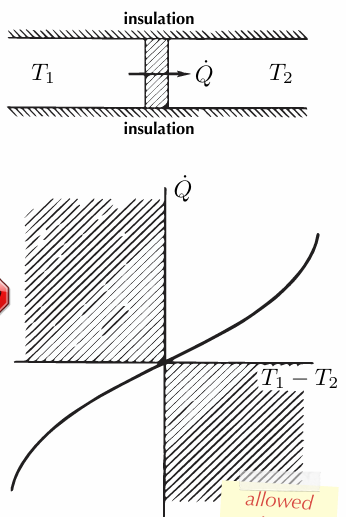
\includegraphics[width=0.5\textwidth]{figs/chapter8/8_2.png}
  \caption{Two perfectly insulated thermal reservoirs at temperatures $T_{1}$ and
  $T_{2}$ ($T_{1} > T_{2}$) connected by a thermal resistor}
\end{figure}

Since the same heat $\dot{Q}$ leaves reservoir 1 and enters reservoir 2,
the power balance at each reservoir gives:
\begin{equation}
  T_{1}\dot{S}_{1} = \dot{Q} = T_{2}\dot{S}_{2}.
  \label{eq:heat_balance}
\end{equation}
The \textbf{net entropy production rate} in the resistor is:
\begin{equation}
  \dot{S}_{2} - \dot{S}_{1}
  = \frac{\dot{Q}}{T_{2}} - \frac{\dot{Q}}{T_{1}}
  = \dot{Q}\,\frac{T_{1} - T_{2}}{T_{1}T_{2}} \geq 0,
  \label{eq:entropy_production}
\end{equation}
which is always non-negative (zero only when $T_{1} = T_{2}$), confirming
the second law.  The entropy flow \emph{leaving} the field is
\emph{greater} than the entropy flow \emph{entering}, regardless of the
direction of heat flow.  This means the thermal resistor is neither a
transformer nor a gyrator: it is an \emph{entropy-generating} element
whose entropy production is independent of the sign of the heat flow.

The thermal resistor is modelled as a \textbf{2-port R-field}:
\begin{equation}
  \frac{T_{1}}{\dot{S}_{1}} \quad R \quad \frac{T_{2}}{\dot{S}_{2}}
  \label{eq:thermal_R}
\end{equation}
This representation differs fundamentally from the pseudo-bond-graph
treatment, where a single scalar resistance connected temperatures and heat
flows.  Here the two entropy-flow ports must be tracked separately because
$\dot{S}_{1} \neq \dot{S}_{2}$.

\begin{insightbox}[The electrical RC analogy has limits]
  It is tempting to model a thermal system exactly like an electrical RC
  network, replacing voltage by temperature and current by heat flow.  This
  analogy is useful but \emph{not} complete: in an electrical resistor the
  current entering equals the current leaving, while in a thermal resistor
  the entropy leaving exceeds the entropy entering.  The analogy between
  electrical and thermal RC systems is therefore not as complete as is often
  assumed.
\end{insightbox}

\paragraph{Constitutive law for the thermal resistor.}
A natural and physically consistent choice is:
\begin{equation}
  \dot{Q} = H(T_{1} - T_{2}),
  \label{eq:thermal_law}
\end{equation}
where $H > 0$ is the \textbf{heat transfer coefficient}.  The individual
entropy flow rates follow from~\eqref{eq:heat_balance}:
\begin{equation}
  \dot{S}_{1} = \frac{H(T_{1} - T_{2})}{T_{1}},
  \qquad
  \dot{S}_{2} = \frac{H(T_{1} - T_{2})}{T_{2}}.
  \label{eq:entropy_rates}
\end{equation}
The \textbf{only admissible causal form} has both temperatures ($T_{1}$ and
$T_{2}$) as inputs and both entropy flows ($\dot{S}_{1}$ and $\dot{S}_{2}$)
as outputs: we cannot impose arbitrary entropy flow rates, because the
constitutive relation~\eqref{eq:entropy_rates} must hold and temperatures
can never be negative.


\subsection{Two compressible chambers: a worked example}
\label{ssec:two_chambers}

As a worked example, consider a system incorporating \textbf{two chambers
containing compressible fluids}:
\begin{itemize}[leftmargin=2em,itemsep=2pt]
  \item One chamber has \emph{constant volume} (the gas is heated or
    cooled only through the thermal resistance).
  \item The other chamber has a \emph{variable volume} whose boundary
    is a piston of area $A$ that can move.
\end{itemize}
The two chambers are separated by the thermal resistance $R$.  The
constitutive laws for the fluids are derived from the total internal energy
$U(S, V)$ of the perfect gas --- specifically, temperature $T$ and pressure
$p$ are found by differentiating $U$ with respect to $S$ and $V$
respectively.

\begin{figure}
  \centering
  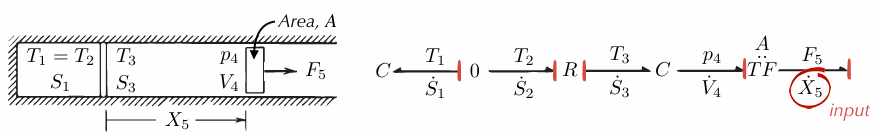
\includegraphics[width=1.0\textwidth]{figs/chapter8/8_3.png}
  \caption{Two-chamber system}
\end{figure}


The model represented by this bond graph is appropriate only for
\textbf{slow changes}: the pseudo-equilibrium assumption requires that
processes occur slowly enough for temperature to be uniform throughout each
chamber at each instant.

Although the entire system is \textbf{power conservative} (no energy is
created or destroyed), the entropy of the two C-elements increases over
time: it appears as if energy is lost.  What the bond graph reveals is that
energy is \emph{not} lost, but rather converted into thermal energy that
\emph{cannot be completely converted back} into mechanical energy --- a
direct manifestation of the second law.  The unique limiting case in which
$X_{5}$ moves so slowly that $T_{2}$ and $T_{3}$ are virtually identical is
the only scenario in which net entropy production almost vanishes.


\subsection{Including Coulomb friction}
\label{ssec:coulomb_friction}

Let us extend the two-chamber model to include \textbf{Coulomb friction}
in the piston.  The friction force is:
\begin{equation}
  F_{6} = A\,\mathrm{sgn}\,\dot{X}_{5},
  \label{eq:coulomb}
\end{equation}
so the dissipated mechanical power is:
\begin{equation}
  F_{6}\dot{X}_{5} = A\dot{X}_{5}\,\mathrm{sgn}\,\dot{X}_{5}
  = A|\dot{X}_{5}| \geq 0.
  \label{eq:friction_power}
\end{equation}
This power is converted entirely into entropy flowing into the adjacent
fluid at temperature $T_{3}$:
\begin{equation}
  \dot{S}_{4} = \frac{1}{T_{3}}\,A|\dot{X}_{5}| \geq 0.
  \label{eq:friction_entropy}
\end{equation}
In bond-graph terms, the mechanical friction is represented as a
\textbf{2-port R-field} connecting a mechanical port and a thermal port.
The R-field can accept either causality at the mechanical port (force or
velocity input), but \emph{only the causality shown} at the thermal port
--- temperature must be an input and entropy flow an output.  The
frictional energy reaches the fluid instantaneously, which is an
idealisation valid when thermal conduction within the fluid is fast
compared to the timescale of interest.


\subsection{Electrothermal resistor}
\label{ssec:electrothermal}

Power dissipation results in thermal effects.  To illustrate the true
bond-graph treatment of mixed energy domains, consider a resistor that
simultaneously carries \textbf{electrical current} and is heated by
\textbf{Joule losses}.  The resistor has a uniform temperature $T$ and
dissipates electrical power:
\begin{equation}
  ei \geq 0,
  \label{eq:joule_positive}
\end{equation}
where $e$ is the voltage and $i$ the current.  If this inequality holds
then both $e$ and $i$ have a ``some'' temperature dependence, because the
resistance is a function of $T$.  The power lost electrically is entirely
converted into heat:
\begin{equation}
  ei = \dot{Q} = T\dot{S}.
  \label{eq:joule_to_heat}
\end{equation}
The R-field has two ports: one electrical ($e$, $i$) and one thermal ($T$,
$\dot{S}$).  There are \textbf{two admissible causal forms}:
\begin{align}
  \text{(a)}\quad e &= e(i, T), &\dot{S} &= \frac{i\,e(i,T)}{T},
  \label{eq:R_causal_a}\\
  \text{(b)}\quad i &= i(e, T), &\dot{S} &= \frac{e\,i(e,T)}{T}.
  \label{eq:R_causal_b}
\end{align}

The temperature of the resistor depends on how much thermal energy has been
stored, so a \textbf{1-port C-element} is necessary to model the thermal
capacity.  It is common to assume $T$ is a linear function of the stored
energy $Q$:
\begin{equation}
  T = T_{0} + \frac{Q}{C},
  \label{eq:T_linear_Q}
\end{equation}
with $\dot{Q} = T\dot{S}$.  However, for the true bond-graph C-element the
constitutive law must express $T$ as a function of the \emph{entropy} $S$:
\begin{equation}
  S = \int_{0}^{S}\mathrm{d}\sigma
  = \int_{0}^{Q}\frac{\mathrm{d}q}{T_{0} + q/C}
  = C\ln\!\left[\frac{1}{T_{0}}\!\left(T_{0} + \frac{Q}{C}\right)\right].
  \label{eq:S_from_Q}
\end{equation}
Inverting gives the true C-field constitutive law:
\begin{equation}
  T = T_{0}\,\mathrm{e}^{S/C},
  \label{eq:T_from_S}
\end{equation}
which is the correct entropy-based form.  Note the nonlinearity: even in
the simple case of constant heat capacity $C$, the true bond-graph
description requires an exponential constitutive law, not a linear one.

\bigskip
\figplaceholder{%
  : the electrical R-field
  (effort $e$, flow $i$) is connected via a 0-junction to the thermal
  C-element (effort $T$, flow $\dot{S}$), with an ambient temperature
  source $T_{0}$ connected via a further R-field representing heat leakage
  to the environment.  Two causal forms of the R-field are shown side by
  side.  Note that the coupling to the ambient can be removed if the
  temperature dependence of the resistance is negligible.}{%
  Slide~17, pack~M08a.}
\bigskip

\begin{figure}
  \centering
  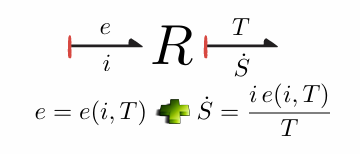
\includegraphics[width=0.6\textwidth]{figs/chapter8/8_4.png}
  \caption{Bond graph for the electrothermal resistor}
\end{figure}


\begin{warningbox}[Only closed systems so far]
  Up to this point, only \textbf{closed systems} have been modelled ---
  no mass crossed the system boundary.  When mass can flow into and out of
  a control volume, the situation becomes significantly more complex and
  requires the introduction of enthalpy convection terms.  This is addressed
  in Section~\ref{ssec:open_volume}.
\end{warningbox}


\subsection{The missing element: no thermal inertia}
\label{ssec:missing_element}

In every energy domain encountered so far (mechanical, electrical,
hydraulic) there is an I-element dual to the C-element.  Let us ask whether
a \textbf{thermal I-element} exists.  In the thermodynamic domain the effort
is temperature $T$ (or temperature difference $\Delta T$) and the flow is
the entropy flow $\dot{S}$.  A hypothetical I-element would obey:
\begin{equation}
  \Delta T = I\,\frac{\mathrm{d}f}{\mathrm{d}t},
  \label{eq:thermal_inertia}
\end{equation}
where $I$ is some parameter (a ``thermal inductance'').
Equation~\eqref{eq:thermal_inertia} implies that $f = \dot{S}$ may have a
\emph{constant non-zero value} even when $\Delta T = 0$: there would be a
sustained entropy (heat) flow in the absence of any temperature difference.

However, the \textbf{second law of thermodynamics} states that a
\emph{spontaneous} heat or entropy flow is \emph{always} directed from a
point of higher temperature to a point of lower temperature.  With an
entropy flow there \emph{must} be a temperature difference.  A thermal
I-element would violate this postulate.  Therefore, \textbf{the I-element
does not exist in the thermodynamic domain}.  This is not a modelling
choice but a fundamental physical constraint.

\begin{insightbox}[``Spontaneous'' means no cross-effects]
  The word ``spontaneous'' in the second-law statement means that no other
  gradients (chemical potential, electric field, etc.) are present that
  might cause cross-effects and drive entropy flow in the absence of a
  temperature difference.  Cross-effects (e.g.\ the Seebeck effect) can
  couple entropy flow to non-thermal driving forces, but these are modelled
  by multi-port elements, not by a thermal I-element.
\end{insightbox}


%──────────────────────────────────────────────────────────────────────
\section{Fluid-dynamic systems revisited}
\label{sec:fluid_revisited}
%──────────────────────────────────────────────────────────────────────

\subsection{Scope and limitations of the bond-graph approach}
\label{ssec:fluid_scope}

The bond-graph models of fluid systems introduced earlier were of the
\textbf{closed-circuit hydraulic type}: static pressure times volume flow
rate ($pQ$) represents most of the transmitted power.  We now take a deeper
look at fluid systems in general and identify the limitations of these
models.

Full \textbf{fluid mechanics} deals with field problems in two or three
dimensions described by PDEs (Navier--Stokes equations), for which
finite-difference or finite-element techniques are required and bond graphs
offer little advantage.  The focus here is therefore:
\begin{itemize}[leftmargin=2em,itemsep=2pt]
  \item The \emph{rough lumping} appropriate when a fluid sub-system is a
    small part of a larger mechatronic system.
  \item \emph{Interior flows} and the fluid-dynamic interaction with solid
    mechanical elements.
\end{itemize}


\subsection{Estimating fluid inertia}
\label{ssec:fluid_inertia}

The I-element represents the inertia of the fluid column.  An elementary
derivation starts from the 1-D assumption: treat the fluid as moving like
a rigid body (quasi-one-dimensional flow) with uniform velocity
$Q/A$ across the cross-section.  Newton's second law for the fluid column of
length $L$ and area $A$ gives:
\begin{equation}
  \rho A L\,\frac{\mathrm{d}}{\mathrm{d}t}\!\left(\frac{Q_{2}}{A}\right)
  = A(p_{1} - p_{3}) = Ap_{2},
  \label{eq:fluid_newton}
\end{equation}
which can be rearranged to:
\begin{equation}
  Q_{2} = \frac{1}{\rho L/A}\,p_{P_{2}},
  \qquad
  I_{\text{fluid}} = \rho L / A
  \quad\text{(inertia coefficient)}.
  \label{eq:fluid_I}
\end{equation}

Several caveats attach to this result:
\begin{itemize}[leftmargin=2em,itemsep=4pt]
  \item The uniform velocity assumption is valid for \emph{transient}
    conditions only approximately; a correcting factor can improve accuracy.
  \item Unless the fluid is \emph{incompressible}, the density $\rho$ is
    not constant and the two ends of the fluid column do not necessarily
    move with the same velocity.
  \item Momentum fluxes at the pipe ends cancel only when the two ends have
    \emph{identical cross-sectional areas}; this derivation does not
    generalise readily to pipes of varying area.
\end{itemize}

\paragraph{The compliance element $C_{6}$.}
The compliance element models the combined compliance of the fluid and pipe
walls.  For small pressure changes the linear capacitor relation is
adequate:
\begin{equation}
  p_{6}(t) = p_{6}(0) + \frac{B}{V_{0}}\int_{0}^{t} Q_{6}\,\mathrm{d}\tau
  = p_{6}(0) + \frac{B}{V_{0}}\,V_{6}(t),
  \label{eq:compliance}
\end{equation}
where $B$ is the bulk modulus and $V_{0}$ the nominal volume.  For
\emph{large} density changes the thermodynamics of the situation must be
studied --- replacing the linear law with a nonlinear one requires a full
thermodynamic analysis (see Section~\ref{ssec:compressible}).

\paragraph{The friction element $R_{4}$.}
The friction element $R_{4}$ represents a pressure loss.  The relation
between $p_{4}$ and $Q_{4}$ is in general \emph{nonlinear}: friction
factor data from experimental fluid mechanics are almost exclusively for
\emph{fully developed steady flow}, making the transient nonlinear
behaviour difficult to capture accurately within a simple lumped model.


\subsection{Bernoulli's equation from the bond-graph viewpoint}
\label{ssec:bernoulli}

To understand the connection between standard fluid mechanics and lumped
bond-graph representation, we derive \textbf{Bernoulli's equation} for
quasi-one-dimensional flow.  This is an extension of the models of M03
and does not involve thermodynamic effects.

We adopt the \textbf{Eulerian method}: let $s$ denote the arc-length
coordinate along the pipe centreline, $v(s,t)$ the average fluid velocity,
$p(s,t)$ the pressure, $A(s)$ the cross-sectional area, and $z(s)$ the
height above a datum.

\begin{figure}
  \centering
  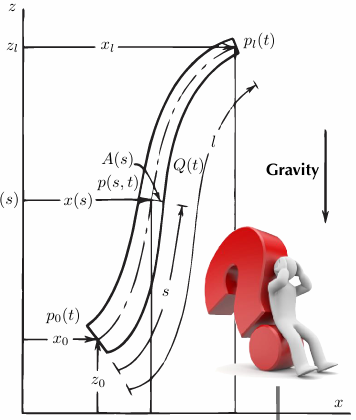
\includegraphics[width=0.4\textwidth]{figs/chapter8/8_5.png}
  \caption{Pipe of varying cross-section}
\end{figure}

\textbf{Newton's law} applied to a fluid element gives the Euler equation
(the \emph{material derivative} $D/Dt$ accounts for both local and
convective acceleration):
\begin{equation}
  \rho\,\frac{Dv}{Dt}
  = \rho\,\frac{\partial v}{\partial t} + \rho v\,\frac{\partial v}{\partial s}
  = -\frac{\partial p}{\partial s} - \rho g\,\frac{\mathrm{d}z}{\mathrm{d}s}.
  \label{eq:euler_eq}
\end{equation}
For an \textbf{incompressible fluid}, continuity requires a constant flow
rate along the pipe:
\begin{equation}
  v(s,t) = \frac{Q(t)}{A(s)}.
  \label{eq:incomp}
\end{equation}
Substituting~\eqref{eq:incomp} into~\eqref{eq:euler_eq} and integrating
along the pipe from $s=0$ to $s=l$:
\begin{equation}
  \rho\left[
    \frac{\dot{Q}(t)}{A(s)}
    + \frac{Q^{2}(t)}{A(s)}\,\frac{\mathrm{d}}{\mathrm{d}s}\!\left(\frac{1}{A(s)}\right)
  \right]
  = -\frac{\partial p}{\partial s} - \rho g\,\frac{\mathrm{d}z}{\mathrm{d}s},
\end{equation}
which integrates to the \textbf{generalised Bernoulli equation}:
\begin{equation}
  \boxed{
    I\dot{Q} + \frac{\rho Q^{2}}{2}\!\left(\frac{1}{A_{l}^{2}} - \frac{1}{A_{0}^{2}}\right)
    = p_{0}(t) - p_{l}(t) - \rho g(z_{l} - z_{0})
  },
  \qquad
  I = \rho\int_{0}^{l}\frac{\mathrm{d}s}{A(s)}.
  \label{eq:bernoulli_bg}
\end{equation}
The first term is the inertia ($I$, with the fluid inertia coefficient
matching~\eqref{eq:fluid_I} for constant $A$); the second term involves
$Q^{2}$ and requires further discussion.


\subsection{Dynamic pressure and the Bernoulli resistance}
\label{ssec:bernoulli_resistance}

The $Q^{2}$ term in~\eqref{eq:bernoulli_bg} is the \textbf{dynamic
pressure} term:
\begin{equation}
  p_{\mathrm{dyn}} = \frac{\rho Q^{2}}{2}\!\left(\frac{1}{A_{l}^{2}} - \frac{1}{A_{0}^{2}}\right).
  \label{eq:dynamic_pressure}
\end{equation}
If $A(s)$ is constant, this term vanishes (the kinetic energies at inlet
and outlet are equal).  When $A$ varies, the term represents the
conversion of static pressure to kinetic energy (nozzle) or vice versa
(diffuser), and is represented in the bond graph as a
\textbf{Bernoulli resistance} $R_{B}$.

This resistance is \emph{unusual}: no matter whether $A_{0} > A_{l}$ or
$A_{0} < A_{l}$, there exist regimes in which $R_{B}$ \emph{appears to supply}
rather than dissipate power.  Furthermore, although the pressure $p_{\mathrm{dyn}}$
is uniquely determined for a given flow rate $Q$, given a pressure
$p_{\mathrm{dyn}}$ there is \emph{either no} corresponding flow rate \emph{or
two} of them --- making the inverse causality (pressure input, flow output)
problematic.  This gives rise to a \textbf{strong preference for the
flow-input causality} when the Bernoulli resistance is included in a bond
graph.

\begin{figure}
  \centering
  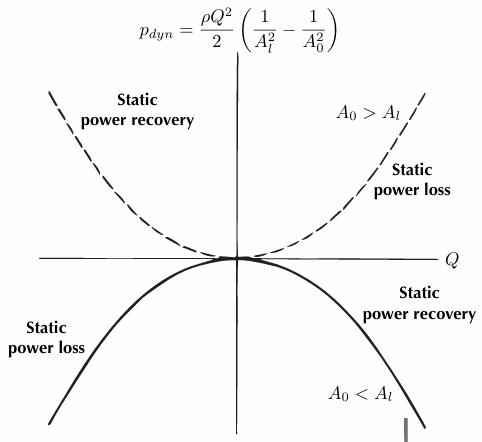
\includegraphics[width=0.4\textwidth]{figs/chapter8/8_6.png}
  \caption{The Bernoulli resistance characteristic}
\end{figure}


\subsection{Example: tank emptying through a pipe}
\label{ssec:tank_emptying}

To illustrate the utility of the bond-graph representation, consider
estimating the time for a \textbf{tank to empty through a pipe}.  The system
consists of a large tank (area $A_{T}$, volume $V$) connected to a pipe of
length $L$ and exit area $A_{2} \ll A_{1} \approx A_{T}$.  The pipe
discharges to a zero-pressure environment ($p_{L} = 0$).

The key assumption is that the fluid fills the pipe at all times ($v = Q/A$),
and the derived equations are valid for \emph{one direction of flow only}.

The bond-graph state equations, derived from~\eqref{eq:bernoulli_bg} with a
Bernoulli resistance and a fluid inertia $I = \rho L/A_{2}$, are:
\begin{align}
  \dot{V} &= -\frac{A_{2}}{\rho L}\,p_{p}, \qquad V \geq 0,
  \label{eq:tank_V}\\
  \dot{p}_{p} &= -\frac{\rho}{2A_{2}^{2}}\!\left(\frac{A_{2}}{\rho L}p_{p}\right)^{2}
  + \frac{\rho g V}{A_{T}}.
  \label{eq:tank_p}
\end{align}
Eliminating $p_{p}$ in favour of $V$:
\begin{equation}
  -\frac{\rho L}{A_{2}}\,\ddot{V}
  = -\frac{\rho}{2A_{2}^{2}}\,\dot{V}^{2} + \frac{\rho g}{A_{T}}\,V,
  \qquad V \geq 0.
  \label{eq:tank_ode}
\end{equation}
This is a second-order nonlinear ODE that can be integrated numerically.
Note that, although no static pressure power flows into the zero-pressure
source at the pipe exit, there \emph{is} a flow; with a diffuser at the
exit one could theoretically recover power from this flow.

\begin{figure}
  \centering
  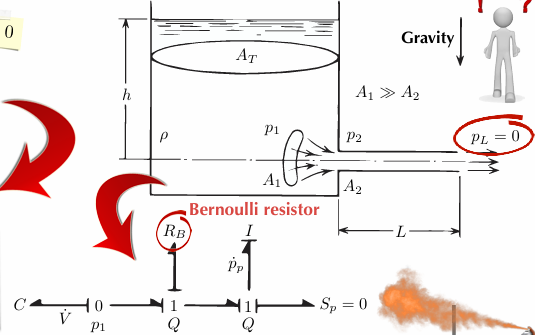
\includegraphics[width=0.4\textwidth]{figs/chapter8/8_7.png}
  \caption{Tank emptying}
\end{figure}


\subsection{Compressible fluids and the transition to pseudo-bond graphs}
\label{ssec:compressible}

For \textbf{small density changes} compressibility is readily modelled by
linear capacitors (as in~\eqref{eq:compliance}).  For
\textbf{large density changes} the thermodynamics of the fluid must be
studied explicitly.  Maintaining a true bond-graph representation for
compressible fluids leads to further complications; this fact motivates the
development of a new form of \textbf{pseudo-bond graph}.

The internal energy per unit mass depends on density $\rho$ and entropy $s$
through the Gibbs equation:
\begin{equation}
  \mathrm{d}u = T\,\mathrm{d}s - p\,\mathrm{d}\!\left(\frac{1}{\rho}\right),
  \qquad
  u = u\!\left(s, \frac{1}{\rho}\right),
  \label{eq:u_rho}
\end{equation}
where $1/\rho$ plays the role of specific volume.  This corresponds to a
C-field in the thermodynamic sense.  Using the C-field representation it is
straightforward to model \emph{closed} systems in which fixed amounts of a
fluid are compressed, expanded, and heated.  When the fluid
\textbf{passes into and out of a control volume} the situation is more
complex.


\subsection{Open volume: convection of internal energy}
\label{ssec:open_volume}

Consider a fluid compressed in a \textbf{fixed volume} $V_{0}$ by allowing
it to pass slowly in and out of a port with volumetric flow rate $Q$ and
pressure $p$:
\begin{equation}
  \rho = \frac{m}{V_{0}}, \qquad \dot{m} = \rho Q.
  \label{eq:open_density}
\end{equation}
The total energy $U$ in the control volume depends on the mass $m$ and the
internal energy per unit mass $u$.  Since $U$ changes not only because of
the \emph{flow work} $pQ$ but also because of the \emph{convection of
internal energy}, the correct flow variable is the \textbf{mass flow rate}
$\dot{m} = \rho Q$.  The energy balance is:
\begin{equation}
  \mathrm{d}U = u\,\mathrm{d}m + \frac{p}{\rho}\,\mathrm{d}m
  = h\,\mathrm{d}m,
  \qquad
  h = u + \frac{p}{\rho}
  \quad\text{(specific enthalpy)},
  \label{eq:dU_enthalpy}
\end{equation}
so that the power entering the control volume is:
\begin{equation}
  h\dot{m} = u\dot{m} + \frac{p}{\rho}\dot{m}
  = u\rho Q + \frac{p}{\rho}\,\rho Q
  = (\rho u + p)Q.
  \label{eq:enthalpy_power}
\end{equation}
In bond-graph terms, it is necessary to \textbf{supplement the pressure}
with an extra term $\rho u$ to account for the convected internal energy.
This is modelled by a \textbf{modulated transformer} (MTF) whose modulus is
$\rho$, converting the port $(p + \rho u,\, Q)$ to the port
$(h,\, \dot{m} = \rho Q)$, which then drives the C-field of the control
volume:

\begin{figure}
  \centering
  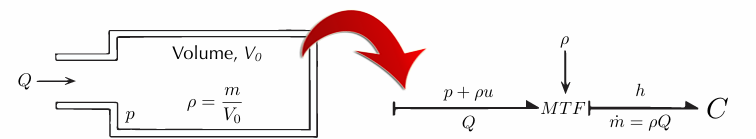
\includegraphics[width=1.0\textwidth]{figs/chapter8/8_8.png}
  \caption{Bond graph for a fixed-volume open control volume}
\end{figure}


\begin{insightbox}[Dynamic pressure neglected]
  The derivation above has \emph{not} incorporated the dynamic pressure term
  $\rho Q^{2}/(2A^{2})$.  The model is therefore valid only for low flow
  rates where the kinetic energy of the incoming stream is negligible
  compared to its enthalpy.
\end{insightbox}

In the \textbf{isentropic case} ($\dot{s} = 0$) pressure and internal
energy are determined solely by the density, so the enthalpy at the port is
determined entirely by conditions \emph{inside} the vessel.  In more
complicated cases (non-isentropic flow) the enthalpy at the port is
determined by:
\begin{itemize}[leftmargin=2em,itemsep=2pt]
  \item Conditions \emph{inside} the vessel for \emph{outflow}.
  \item \emph{External} conditions for \emph{inflow}.
\end{itemize}
This causal switching with changes in the direction of flow is not readily
apparent in the true bond graph; it will be explicitly addressed in the
pseudo-bond-graph formulations developed in the following chapters.


\subsection{Variable-volume compression: the piston--cylinder}
\label{ssec:piston_cylinder}

As a final extension, consider \textbf{isentropic compression} occurring
simultaneously due to variable volume (a piston) and to inflow/outflow.
The cylinder has area $A$, piston displacement $x$, and volume $V = Ax$.
The total energy $U$ depends on both the mass $m$ and the volume $V$, so
the C-field satisfies:
\begin{equation}
  h = \frac{\partial U}{\partial m},
  \qquad
  -p = \frac{\partial U}{\partial V}.
  \label{eq:piston_cfield}
\end{equation}
The bond graph is a more sophisticated version of the compressibility models
used in servomechanisms, where the volume of fluid is variable.

\begin{figure}
  \centering
  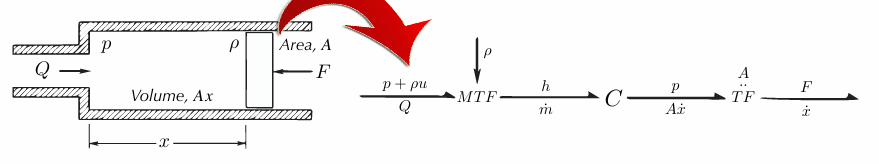
\includegraphics[width=1.0\textwidth]{figs/chapter8/8_9.png}
  \caption{Piston--cylinder with inflow/outflow}
\end{figure}

This bond graph is a powerful, general representation: it handles
simultaneously the thermodynamics of compression, the convection of mass and
energy through the port, and the mechanical work done by or on the piston.
Linearised compressibility parameters (constant bulk modulus) are a special
case, but it is \textbf{virtually impossible} to proceed from a linearised
model to a more accurate nonlinear one without returning to the physics and
reconstructing the bond graph from scratch.  The systematic derivation from
$U(m, V)$ ensures that the nonlinear model is available from the outset and
that no energy-conservation errors are introduced by \emph{ad hoc}
linearisation.

%──────────────────────────────────────────────────────────────────────
\section{Summary}
\label{sec:thermofluid_summary}
%──────────────────────────────────────────────────────────────────────

This chapter has developed the bond-graph treatment of thermo-fluid systems
at two levels of depth.

\paragraph{True bond graphs for thermodynamics.}
The pure substance is a 2-port C-field with $T$ (effort) and $\dot{s}$
(flow) at one port and $p$ (effort) and $\dot{v}$ (flow) at the other.  The
product $T\dot{s}$ is genuine thermodynamic power.  The four causal
patterns of this C-field correspond to the four classical thermodynamic
potentials ($u$, $h$, $f$, $\phi$) via Legendre transformations, and all
four automatically ensure conservation of energy.  Heat transfer is modelled
by a 2-port R-field that generates entropy; its only admissible causality
has temperatures as inputs.  A thermal I-element is physically impossible
(it would violate the second law).  With these elements a rich variety of
thermal and electrothermal systems can be modelled rigorously.

\paragraph{Fluid-dynamic lumped models.}
Standard lumped models of fluid systems (fluid inertia $I = \rho L/A$,
compliance $B/V_{0}$, friction $R$, leakage $R$) are useful for short,
linear elements but carry significant philosophical caveats for long pipes,
nonlinear flows, and compressible fluids.  The Bernoulli equation reveals
an unusual $Q^{2}$ term (dynamic pressure / Bernoulli resistance) that
can supply as well as dissipate power and creates multi-valuedness under
pressure-input causality.  For compressible fluids with mass exchange
through a control volume, the correct power variable at the port is the
enthalpy flux $h\dot{m}$, and the bond graph requires an MTF to account for
convected internal energy.  The resulting nonlinear C-field formulation is
the natural starting point for accurate models of pneumatic actuators,
compressors, and variable-volume reservoirs.